\documentclass[aspectratio=169]{beamer}
\usepackage[utf8]{inputenc}
\usefonttheme{serif} 
\usefonttheme{structuresmallcapsserif} 
\usepackage{hyperref}
\hypersetup{
    colorlinks=true,
    linkcolor=blue,
    filecolor=magenta,      
    urlcolor=cyan,
}

\usetheme{Luebeck}
\usepackage{multimedia}
\usepackage{textpos} 

\addtobeamertemplate{frametitle}{}{%
    \begin{textblock*}{100mm}(11.75cm,-0.86cm)
        
\includegraphics[height=0.86cm,width=0.86cm]{HIPlogo.png}
    \end{textblock*}
    }
\addtobeamertemplate{frametitle}{}{%
    \begin{textblock*}{100mm}(10.89cm,-0.86cm)
        
\includegraphics[height=0.86cm,width=0.86cm]{HYlogo.jpg}
    \end{textblock*}}
\addtobeamertemplate{frametitle}{}{%
    \begin{textblock*}{100mm}(10.03cm,-0.86cm)
        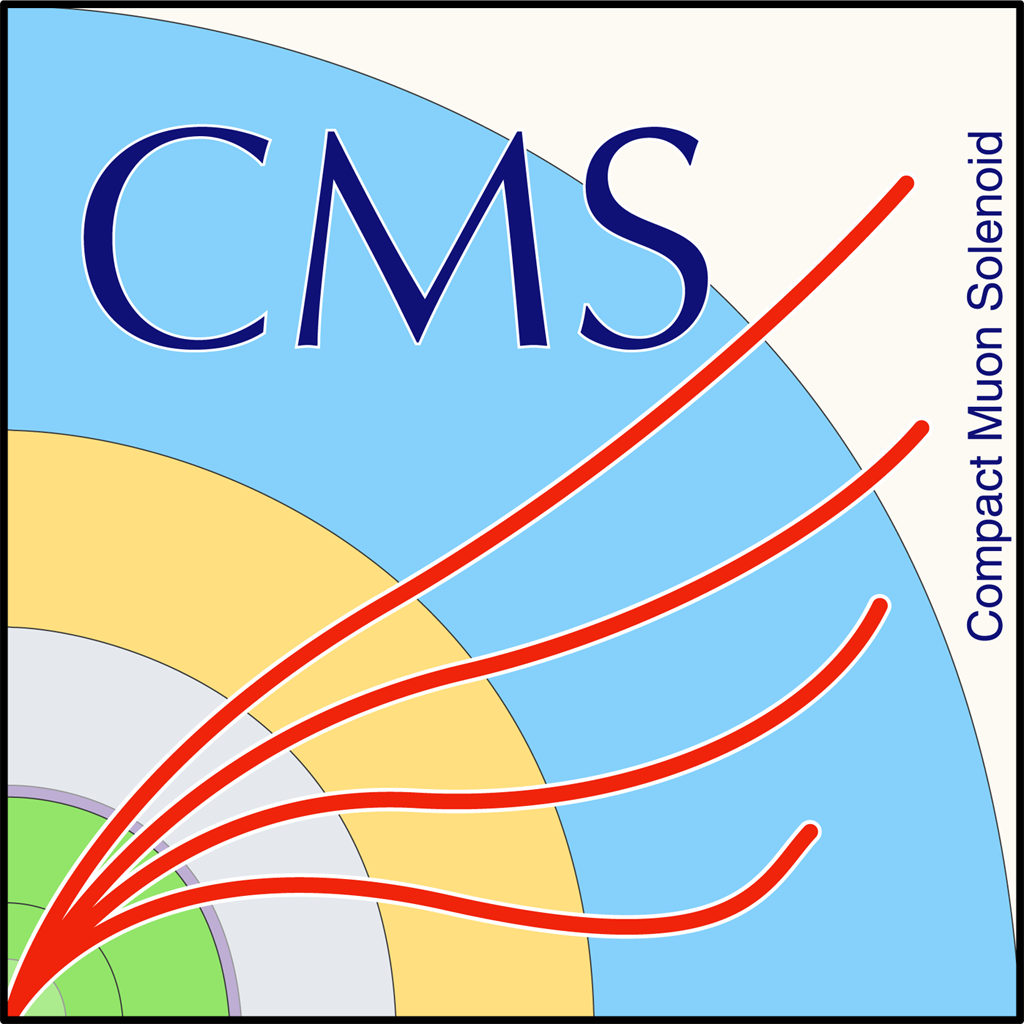
\includegraphics[height=0.86cm,width=0.86cm]{CMSlogo.png}
    \end{textblock*}}

\definecolor{ao}{rgb}{0.0, 0.5, 0.0}
\definecolor{darkgreen}{rgb}{0.0, 0.2, 0.13}
\definecolor{ferngreen}{rgb}{0.31, 0.47, 0.26}
    
\usecolortheme[named=ferngreen]{structure}
\beamertemplatenavigationsymbolsempty
\setbeamertemplate{bibliography item}[text]
\title[Legacy data jet energy fractions vs pt]{Legacy data jet energy fractions vs pt}
\author{Hannu Siikonen}
\institute{Helsinki Institute of Physics \\ \vspace{0.25cm} Instructor Adj.~Prof.~Mikko~Voutilainen}

\date{\today}

\setbeamersize{text margin left=0.5pt,text margin right=-3pt}
\setlength{\labelsep}{12pt}

\begin{document}

\titlepage

\newpage

\begin{figure}[p]
\flushleft
\begin{columns}[T]
\begin{column}{.2\linewidth}
\centering
All trigs poseta
\end{column}
\begin{column}{.8\linewidth}
\includegraphics[width=0.20\paperwidth]{../pypdf/drawFracs_vsphipos_0-13.pdf}
\includegraphics[width=0.20\paperwidth]{../pypdf/drawFracs_vsphipos_0-5.pdf}
\includegraphics[width=0.20\paperwidth]{../pypdf/drawFracs_vsphipos_5-10.pdf}
\includegraphics[width=0.20\paperwidth]{../pypdf/drawFracs_vsphipos_10-15.pdf}
\end{column}
\end{columns}
\includegraphics[width=0.20\paperwidth]{../pypdf/drawFracs_vsphipos_15-20.pdf}
\includegraphics[width=0.20\paperwidth]{../pypdf/drawFracs_vsphipos_20-25.pdf}
\includegraphics[width=0.20\paperwidth]{../pypdf/drawFracs_vsphipos_25-30.pdf}
\includegraphics[width=0.20\paperwidth]{../pypdf/drawFracs_vsphipos_30-32.pdf}
\includegraphics[width=0.20\paperwidth]{../pypdf/drawFracs_vsphipos_32-47.pdf}
\end{figure}


\begin{figure}[p]
\flushleft
\begin{columns}[T]
\begin{column}{.2\linewidth}
\centering
All trigs negeta
\end{column}
\begin{column}{.8\linewidth}
\includegraphics[width=0.20\paperwidth]{../pypdf/drawFracs_vsphineg_0-13.pdf}
\includegraphics[width=0.20\paperwidth]{../pypdf/drawFracs_vsphineg_0-5.pdf}
\includegraphics[width=0.20\paperwidth]{../pypdf/drawFracs_vsphineg_5-10.pdf}
\includegraphics[width=0.20\paperwidth]{../pypdf/drawFracs_vsphineg_10-15.pdf}
\end{column}
\end{columns}
\includegraphics[width=0.20\paperwidth]{../pypdf/drawFracs_vsphineg_15-20.pdf}
\includegraphics[width=0.20\paperwidth]{../pypdf/drawFracs_vsphineg_20-25.pdf}
\includegraphics[width=0.20\paperwidth]{../pypdf/drawFracs_vsphineg_25-30.pdf}
\includegraphics[width=0.20\paperwidth]{../pypdf/drawFracs_vsphineg_30-32.pdf}
\includegraphics[width=0.20\paperwidth]{../pypdf/drawFracs_vsphineg_32-47.pdf}
\end{figure}

\begin{figure}[p]
\flushleft
\begin{columns}[T]
\begin{column}{.2\linewidth}
\centering
jt40 poseta
\end{column}
\begin{column}{.8\linewidth}
\includegraphics[width=0.20\paperwidth]{../pypdf/drawFracs_vsphipos_jt40_0-5.pdf}
\includegraphics[width=0.20\paperwidth]{../pypdf/drawFracs_vsphipos_jt40_5-10.pdf}
\includegraphics[width=0.20\paperwidth]{../pypdf/drawFracs_vsphipos_jt40_10-15.pdf}
\includegraphics[width=0.20\paperwidth]{../pypdf/drawFracs_vsphipos_jt40_15-20.pdf}
\end{column}
\end{columns}
\includegraphics[width=0.20\paperwidth]{../pypdf/drawFracs_vsphipos_jt40_0-13.pdf}
\includegraphics[width=0.20\paperwidth]{../pypdf/drawFracs_vsphipos_jt40_20-25.pdf}
\includegraphics[width=0.20\paperwidth]{../pypdf/drawFracs_vsphipos_jt40_25-30.pdf}
\includegraphics[width=0.20\paperwidth]{../pypdf/drawFracs_vsphipos_jt40_30-32.pdf}
\includegraphics[width=0.20\paperwidth]{../pypdf/drawFracs_vsphipos_jt40_32-47.pdf}
\end{figure}
\begin{figure}[p]
\flushleft
\begin{columns}[T]
\begin{column}{.2\linewidth}
\centering
jt40 negeta
\end{column}
\begin{column}{.8\linewidth}
\includegraphics[width=0.20\paperwidth]{../pypdf/drawFracs_vsphineg_jt40_0-5.pdf}
\includegraphics[width=0.20\paperwidth]{../pypdf/drawFracs_vsphineg_jt40_5-10.pdf}
\includegraphics[width=0.20\paperwidth]{../pypdf/drawFracs_vsphineg_jt40_10-15.pdf}
\includegraphics[width=0.20\paperwidth]{../pypdf/drawFracs_vsphineg_jt40_15-20.pdf}
\end{column}
\end{columns}
\includegraphics[width=0.20\paperwidth]{../pypdf/drawFracs_vsphineg_jt40_0-13.pdf}
\includegraphics[width=0.20\paperwidth]{../pypdf/drawFracs_vsphineg_jt40_20-25.pdf}
\includegraphics[width=0.20\paperwidth]{../pypdf/drawFracs_vsphineg_jt40_25-30.pdf}
\includegraphics[width=0.20\paperwidth]{../pypdf/drawFracs_vsphineg_jt40_30-32.pdf}
\includegraphics[width=0.20\paperwidth]{../pypdf/drawFracs_vsphineg_jt40_32-47.pdf}
\end{figure}

\begin{figure}[p]
\flushleft
\begin{columns}[T]
\begin{column}{.2\linewidth}
\centering
jt60 poseta
\end{column}
\begin{column}{.8\linewidth}
\includegraphics[width=0.20\paperwidth]{../pypdf/drawFracs_vsphipos_jt60_0-5.pdf}
\includegraphics[width=0.20\paperwidth]{../pypdf/drawFracs_vsphipos_jt60_5-10.pdf}
\includegraphics[width=0.20\paperwidth]{../pypdf/drawFracs_vsphipos_jt60_10-15.pdf}
\includegraphics[width=0.20\paperwidth]{../pypdf/drawFracs_vsphipos_jt60_15-20.pdf}
\end{column}
\end{columns}
\includegraphics[width=0.20\paperwidth]{../pypdf/drawFracs_vsphipos_jt60_0-13.pdf}
\includegraphics[width=0.20\paperwidth]{../pypdf/drawFracs_vsphipos_jt60_20-25.pdf}
\includegraphics[width=0.20\paperwidth]{../pypdf/drawFracs_vsphipos_jt60_25-30.pdf}
\includegraphics[width=0.20\paperwidth]{../pypdf/drawFracs_vsphipos_jt60_30-32.pdf}
\includegraphics[width=0.20\paperwidth]{../pypdf/drawFracs_vsphipos_jt60_32-47.pdf}
\end{figure}

\begin{figure}[p]
\flushleft
\begin{columns}[T]
\begin{column}{.2\linewidth}
\centering
jt60 negeta
\end{column}
\begin{column}{.8\linewidth}
\includegraphics[width=0.20\paperwidth]{../pypdf/drawFracs_vsphineg_jt60_0-5.pdf}
\includegraphics[width=0.20\paperwidth]{../pypdf/drawFracs_vsphineg_jt60_5-10.pdf}
\includegraphics[width=0.20\paperwidth]{../pypdf/drawFracs_vsphineg_jt60_10-15.pdf}
\includegraphics[width=0.20\paperwidth]{../pypdf/drawFracs_vsphineg_jt60_15-20.pdf}
\end{column}
\end{columns}
\includegraphics[width=0.20\paperwidth]{../pypdf/drawFracs_vsphineg_jt60_0-13.pdf}
\includegraphics[width=0.20\paperwidth]{../pypdf/drawFracs_vsphineg_jt60_20-25.pdf}
\includegraphics[width=0.20\paperwidth]{../pypdf/drawFracs_vsphineg_jt60_25-30.pdf}
\includegraphics[width=0.20\paperwidth]{../pypdf/drawFracs_vsphineg_jt60_30-32.pdf}
\includegraphics[width=0.20\paperwidth]{../pypdf/drawFracs_vsphineg_jt60_32-47.pdf}
\end{figure}

\begin{figure}[p]
\flushleft
\begin{columns}[T]
\begin{column}{.2\linewidth}
\centering
jt80 poseta
\end{column}
\begin{column}{.8\linewidth}
\includegraphics[width=0.20\paperwidth]{../pypdf/drawFracs_vsphipos_jt80_0-5.pdf}
\includegraphics[width=0.20\paperwidth]{../pypdf/drawFracs_vsphipos_jt80_5-10.pdf}
\includegraphics[width=0.20\paperwidth]{../pypdf/drawFracs_vsphipos_jt80_10-15.pdf}
\includegraphics[width=0.20\paperwidth]{../pypdf/drawFracs_vsphipos_jt80_15-20.pdf}
\end{column}
\end{columns}
\includegraphics[width=0.20\paperwidth]{../pypdf/drawFracs_vsphipos_jt80_0-13.pdf}
\includegraphics[width=0.20\paperwidth]{../pypdf/drawFracs_vsphipos_jt80_20-25.pdf}
\includegraphics[width=0.20\paperwidth]{../pypdf/drawFracs_vsphipos_jt80_25-30.pdf}
\includegraphics[width=0.20\paperwidth]{../pypdf/drawFracs_vsphipos_jt80_30-32.pdf}
\includegraphics[width=0.20\paperwidth]{../pypdf/drawFracs_vsphipos_jt80_32-47.pdf}
\end{figure}

\begin{figure}[p]
\flushleft
\begin{columns}[T]
\begin{column}{.2\linewidth}
\centering
jt80 negeta
\end{column}
\begin{column}{.8\linewidth}
\includegraphics[width=0.20\paperwidth]{../pypdf/drawFracs_vsphineg_jt80_0-5.pdf}
\includegraphics[width=0.20\paperwidth]{../pypdf/drawFracs_vsphineg_jt80_5-10.pdf}
\includegraphics[width=0.20\paperwidth]{../pypdf/drawFracs_vsphineg_jt80_10-15.pdf}
\includegraphics[width=0.20\paperwidth]{../pypdf/drawFracs_vsphineg_jt80_15-20.pdf}
\end{column}
\end{columns}
\includegraphics[width=0.20\paperwidth]{../pypdf/drawFracs_vsphineg_jt80_0-13.pdf}
\includegraphics[width=0.20\paperwidth]{../pypdf/drawFracs_vsphineg_jt80_20-25.pdf}
\includegraphics[width=0.20\paperwidth]{../pypdf/drawFracs_vsphineg_jt80_25-30.pdf}
\includegraphics[width=0.20\paperwidth]{../pypdf/drawFracs_vsphineg_jt80_30-32.pdf}
\includegraphics[width=0.20\paperwidth]{../pypdf/drawFracs_vsphineg_jt80_32-47.pdf}
\end{figure}


\begin{figure}[p]
\flushleft
\begin{columns}[T]
\begin{column}{.2\linewidth}
\centering
jt140 poseta
\end{column}
\begin{column}{.8\linewidth}
\includegraphics[width=0.20\paperwidth]{../pypdf/drawFracs_vsphipos_jt140_0-5.pdf}
\includegraphics[width=0.20\paperwidth]{../pypdf/drawFracs_vsphipos_jt140_5-10.pdf}
\includegraphics[width=0.20\paperwidth]{../pypdf/drawFracs_vsphipos_jt140_10-15.pdf}
\includegraphics[width=0.20\paperwidth]{../pypdf/drawFracs_vsphipos_jt140_15-20.pdf}
\end{column}
\end{columns}
\includegraphics[width=0.20\paperwidth]{../pypdf/drawFracs_vsphipos_jt140_0-13.pdf}
\includegraphics[width=0.20\paperwidth]{../pypdf/drawFracs_vsphipos_jt140_20-25.pdf}
\includegraphics[width=0.20\paperwidth]{../pypdf/drawFracs_vsphipos_jt140_25-30.pdf}
\includegraphics[width=0.20\paperwidth]{../pypdf/drawFracs_vsphipos_jt140_30-32.pdf}
\includegraphics[width=0.20\paperwidth]{../pypdf/drawFracs_vsphipos_jt140_32-47.pdf}
\end{figure}

\begin{figure}[p]
\flushleft
\begin{columns}[T]
\begin{column}{.2\linewidth}
\centering
jt140 negeta
\end{column}
\begin{column}{.8\linewidth}
\includegraphics[width=0.20\paperwidth]{../pypdf/drawFracs_vsphineg_jt140_0-5.pdf}
\includegraphics[width=0.20\paperwidth]{../pypdf/drawFracs_vsphineg_jt140_5-10.pdf}
\includegraphics[width=0.20\paperwidth]{../pypdf/drawFracs_vsphineg_jt140_10-15.pdf}
\includegraphics[width=0.20\paperwidth]{../pypdf/drawFracs_vsphineg_jt140_15-20.pdf}
\end{column}
\end{columns}
\includegraphics[width=0.20\paperwidth]{../pypdf/drawFracs_vsphineg_jt140_0-13.pdf}
\includegraphics[width=0.20\paperwidth]{../pypdf/drawFracs_vsphineg_jt140_20-25.pdf}
\includegraphics[width=0.20\paperwidth]{../pypdf/drawFracs_vsphineg_jt140_25-30.pdf}
\includegraphics[width=0.20\paperwidth]{../pypdf/drawFracs_vsphineg_jt140_30-32.pdf}
\includegraphics[width=0.20\paperwidth]{../pypdf/drawFracs_vsphineg_jt140_32-47.pdf}
\end{figure}

\begin{figure}[p]
\flushleft
\begin{columns}[T]
\begin{column}{.2\linewidth}
\centering
jt200 poseta
\end{column}
\begin{column}{.8\linewidth}
\includegraphics[width=0.20\paperwidth]{../pypdf/drawFracs_vsphipos_jt200_0-5.pdf}
\includegraphics[width=0.20\paperwidth]{../pypdf/drawFracs_vsphipos_jt200_5-10.pdf}
\includegraphics[width=0.20\paperwidth]{../pypdf/drawFracs_vsphipos_jt200_10-15.pdf}
\includegraphics[width=0.20\paperwidth]{../pypdf/drawFracs_vsphipos_jt200_15-20.pdf}
\end{column}
\end{columns}
\includegraphics[width=0.20\paperwidth]{../pypdf/drawFracs_vsphipos_jt200_0-13.pdf}
\includegraphics[width=0.20\paperwidth]{../pypdf/drawFracs_vsphipos_jt200_20-25.pdf}
\includegraphics[width=0.20\paperwidth]{../pypdf/drawFracs_vsphipos_jt200_25-30.pdf}
\includegraphics[width=0.20\paperwidth]{../pypdf/drawFracs_vsphipos_jt200_30-32.pdf}
\includegraphics[width=0.20\paperwidth]{../pypdf/drawFracs_vsphipos_jt200_32-47.pdf}
\end{figure}

\begin{figure}[p]
\flushleft
\begin{columns}[T]
\begin{column}{.2\linewidth}
\centering
jt200 negeta
\end{column}
\begin{column}{.8\linewidth}
\includegraphics[width=0.20\paperwidth]{../pypdf/drawFracs_vsphineg_jt200_0-5.pdf}
\includegraphics[width=0.20\paperwidth]{../pypdf/drawFracs_vsphineg_jt200_5-10.pdf}
\includegraphics[width=0.20\paperwidth]{../pypdf/drawFracs_vsphineg_jt200_10-15.pdf}
\includegraphics[width=0.20\paperwidth]{../pypdf/drawFracs_vsphineg_jt200_15-20.pdf}
\end{column}
\end{columns}
\includegraphics[width=0.20\paperwidth]{../pypdf/drawFracs_vsphineg_jt200_0-13.pdf}
\includegraphics[width=0.20\paperwidth]{../pypdf/drawFracs_vsphineg_jt200_20-25.pdf}
\includegraphics[width=0.20\paperwidth]{../pypdf/drawFracs_vsphineg_jt200_25-30.pdf}
\includegraphics[width=0.20\paperwidth]{../pypdf/drawFracs_vsphineg_jt200_30-32.pdf}
\includegraphics[width=0.20\paperwidth]{../pypdf/drawFracs_vsphineg_jt200_32-47.pdf}
\end{figure}

\begin{figure}[p]
\flushleft
\begin{columns}[T]
\begin{column}{.2\linewidth}
\centering
jt260 poseta
\end{column}
\begin{column}{.8\linewidth}
\includegraphics[width=0.20\paperwidth]{../pypdf/drawFracs_vsphipos_jt260_0-5.pdf}
\includegraphics[width=0.20\paperwidth]{../pypdf/drawFracs_vsphipos_jt260_5-10.pdf}
\includegraphics[width=0.20\paperwidth]{../pypdf/drawFracs_vsphipos_jt260_10-15.pdf}
\includegraphics[width=0.20\paperwidth]{../pypdf/drawFracs_vsphipos_jt260_15-20.pdf}
\end{column}
\end{columns}
\includegraphics[width=0.20\paperwidth]{../pypdf/drawFracs_vsphipos_jt260_0-13.pdf}
\includegraphics[width=0.20\paperwidth]{../pypdf/drawFracs_vsphipos_jt260_20-25.pdf}
\includegraphics[width=0.20\paperwidth]{../pypdf/drawFracs_vsphipos_jt260_25-30.pdf}
\includegraphics[width=0.20\paperwidth]{../pypdf/drawFracs_vsphipos_jt260_30-32.pdf}
\includegraphics[width=0.20\paperwidth]{../pypdf/drawFracs_vsphipos_jt260_32-47.pdf}
\end{figure}


\begin{figure}[p]
\flushleft
\begin{columns}[T]
\begin{column}{.2\linewidth}
\centering
jt260 negeta
\end{column}
\begin{column}{.8\linewidth}
\includegraphics[width=0.20\paperwidth]{../pypdf/drawFracs_vsphineg_jt260_0-5.pdf}
\includegraphics[width=0.20\paperwidth]{../pypdf/drawFracs_vsphineg_jt260_5-10.pdf}
\includegraphics[width=0.20\paperwidth]{../pypdf/drawFracs_vsphineg_jt260_10-15.pdf}
\includegraphics[width=0.20\paperwidth]{../pypdf/drawFracs_vsphineg_jt260_15-20.pdf}
\end{column}
\end{columns}
\includegraphics[width=0.20\paperwidth]{../pypdf/drawFracs_vsphineg_jt260_0-13.pdf}
\includegraphics[width=0.20\paperwidth]{../pypdf/drawFracs_vsphineg_jt260_20-25.pdf}
\includegraphics[width=0.20\paperwidth]{../pypdf/drawFracs_vsphineg_jt260_25-30.pdf}
\includegraphics[width=0.20\paperwidth]{../pypdf/drawFracs_vsphineg_jt260_30-32.pdf}
\includegraphics[width=0.20\paperwidth]{../pypdf/drawFracs_vsphineg_jt260_32-47.pdf}
\end{figure}

\begin{figure}[p]
\flushleft
\begin{columns}[T]
\begin{column}{.2\linewidth}
\centering
jt320 poseta
\end{column}
\begin{column}{.8\linewidth}
\includegraphics[width=0.20\paperwidth]{../pypdf/drawFracs_vsphipos_jt320_0-5.pdf}
\includegraphics[width=0.20\paperwidth]{../pypdf/drawFracs_vsphipos_jt320_5-10.pdf}
\includegraphics[width=0.20\paperwidth]{../pypdf/drawFracs_vsphipos_jt320_10-15.pdf}
\includegraphics[width=0.20\paperwidth]{../pypdf/drawFracs_vsphipos_jt320_15-20.pdf}
\end{column}
\end{columns}
\includegraphics[width=0.20\paperwidth]{../pypdf/drawFracs_vsphipos_jt320_0-13.pdf}
\includegraphics[width=0.20\paperwidth]{../pypdf/drawFracs_vsphipos_jt320_20-25.pdf}
\includegraphics[width=0.20\paperwidth]{../pypdf/drawFracs_vsphipos_jt320_25-30.pdf}
\includegraphics[width=0.20\paperwidth]{../pypdf/drawFracs_vsphipos_jt320_30-32.pdf}
\includegraphics[width=0.20\paperwidth]{../pypdf/drawFracs_vsphipos_jt320_32-47.pdf}
\end{figure}

\begin{figure}[p]
\flushleft
\begin{columns}[T]
\begin{column}{.2\linewidth}
\centering
jt320 negeta
\end{column}
\begin{column}{.8\linewidth}
\includegraphics[width=0.20\paperwidth]{../pypdf/drawFracs_vsphineg_jt320_0-5.pdf}
\includegraphics[width=0.20\paperwidth]{../pypdf/drawFracs_vsphineg_jt320_5-10.pdf}
\includegraphics[width=0.20\paperwidth]{../pypdf/drawFracs_vsphineg_jt320_10-15.pdf}
\includegraphics[width=0.20\paperwidth]{../pypdf/drawFracs_vsphineg_jt320_15-20.pdf}
\end{column}
\end{columns}
\includegraphics[width=0.20\paperwidth]{../pypdf/drawFracs_vsphineg_jt320_0-13.pdf}
\includegraphics[width=0.20\paperwidth]{../pypdf/drawFracs_vsphineg_jt320_20-25.pdf}
\includegraphics[width=0.20\paperwidth]{../pypdf/drawFracs_vsphineg_jt320_25-30.pdf}
\includegraphics[width=0.20\paperwidth]{../pypdf/drawFracs_vsphineg_jt320_30-32.pdf}
\includegraphics[width=0.20\paperwidth]{../pypdf/drawFracs_vsphineg_jt320_32-47.pdf}
\end{figure}

\begin{figure}[p]
\flushleft
\begin{columns}[T]
\begin{column}{.2\linewidth}
\centering
jt400 poseta
\end{column}
\begin{column}{.8\linewidth}
\includegraphics[width=0.20\paperwidth]{../pypdf/drawFracs_vsphipos_jt400_0-5.pdf}
\includegraphics[width=0.20\paperwidth]{../pypdf/drawFracs_vsphipos_jt400_5-10.pdf}
\includegraphics[width=0.20\paperwidth]{../pypdf/drawFracs_vsphipos_jt400_10-15.pdf}
\includegraphics[width=0.20\paperwidth]{../pypdf/drawFracs_vsphipos_jt400_15-20.pdf}
\end{column}
\end{columns}
\includegraphics[width=0.20\paperwidth]{../pypdf/drawFracs_vsphipos_jt400_0-13.pdf}
\includegraphics[width=0.20\paperwidth]{../pypdf/drawFracs_vsphipos_jt400_20-25.pdf}
\includegraphics[width=0.20\paperwidth]{../pypdf/drawFracs_vsphipos_jt400_25-30.pdf}
\includegraphics[width=0.20\paperwidth]{../pypdf/drawFracs_vsphipos_jt400_30-32.pdf}
\includegraphics[width=0.20\paperwidth]{../pypdf/drawFracs_vsphipos_jt400_32-47.pdf}
\end{figure}

\begin{figure}[p]
\flushleft
\begin{columns}[T]
\begin{column}{.2\linewidth}
\centering
jt400 negeta
\end{column}
\begin{column}{.8\linewidth}
\includegraphics[width=0.20\paperwidth]{../pypdf/drawFracs_vsphineg_jt400_0-5.pdf}
\includegraphics[width=0.20\paperwidth]{../pypdf/drawFracs_vsphineg_jt400_5-10.pdf}
\includegraphics[width=0.20\paperwidth]{../pypdf/drawFracs_vsphineg_jt400_10-15.pdf}
\includegraphics[width=0.20\paperwidth]{../pypdf/drawFracs_vsphineg_jt400_15-20.pdf}
\end{column}
\end{columns}
\includegraphics[width=0.20\paperwidth]{../pypdf/drawFracs_vsphineg_jt400_0-13.pdf}
\includegraphics[width=0.20\paperwidth]{../pypdf/drawFracs_vsphineg_jt400_20-25.pdf}
\includegraphics[width=0.20\paperwidth]{../pypdf/drawFracs_vsphineg_jt400_25-30.pdf}
\includegraphics[width=0.20\paperwidth]{../pypdf/drawFracs_vsphineg_jt400_30-32.pdf}
\includegraphics[width=0.20\paperwidth]{../pypdf/drawFracs_vsphineg_jt400_32-47.pdf}
\end{figure}

\begin{figure}[p]
\flushleft
\begin{columns}[T]
\begin{column}{.2\linewidth}
\centering
jt450 poseta
\end{column}
\begin{column}{.8\linewidth}
\includegraphics[width=0.20\paperwidth]{../pypdf/drawFracs_vsphipos_jt450_0-5.pdf}
\includegraphics[width=0.20\paperwidth]{../pypdf/drawFracs_vsphipos_jt450_5-10.pdf}
\includegraphics[width=0.20\paperwidth]{../pypdf/drawFracs_vsphipos_jt450_10-15.pdf}
\includegraphics[width=0.20\paperwidth]{../pypdf/drawFracs_vsphipos_jt450_15-20.pdf}
\end{column}
\end{columns}
\includegraphics[width=0.20\paperwidth]{../pypdf/drawFracs_vsphipos_jt450_0-13.pdf}
\includegraphics[width=0.20\paperwidth]{../pypdf/drawFracs_vsphipos_jt450_20-25.pdf}
\includegraphics[width=0.20\paperwidth]{../pypdf/drawFracs_vsphipos_jt450_25-30.pdf}
\includegraphics[width=0.20\paperwidth]{../pypdf/drawFracs_vsphipos_jt450_30-32.pdf}
\includegraphics[width=0.20\paperwidth]{../pypdf/drawFracs_vsphipos_jt450_32-47.pdf}
\end{figure}

\begin{figure}[p]
\flushleft
\begin{columns}[T]
\begin{column}{.2\linewidth}
\centering
jt450 negeta
\end{column}
\begin{column}{.8\linewidth}
\includegraphics[width=0.20\paperwidth]{../pypdf/drawFracs_vsphineg_jt450_0-5.pdf}
\includegraphics[width=0.20\paperwidth]{../pypdf/drawFracs_vsphineg_jt450_5-10.pdf}
\includegraphics[width=0.20\paperwidth]{../pypdf/drawFracs_vsphineg_jt450_10-15.pdf}
\includegraphics[width=0.20\paperwidth]{../pypdf/drawFracs_vsphineg_jt450_15-20.pdf}
\end{column}
\end{columns}
\includegraphics[width=0.20\paperwidth]{../pypdf/drawFracs_vsphineg_jt450_0-13.pdf}
\includegraphics[width=0.20\paperwidth]{../pypdf/drawFracs_vsphineg_jt450_20-25.pdf}
\includegraphics[width=0.20\paperwidth]{../pypdf/drawFracs_vsphineg_jt450_25-30.pdf}
\includegraphics[width=0.20\paperwidth]{../pypdf/drawFracs_vsphineg_jt450_30-32.pdf}
\includegraphics[width=0.20\paperwidth]{../pypdf/drawFracs_vsphineg_jt450_32-47.pdf}
\end{figure}

\begin{figure}[p]
\flushleft
\begin{columns}[T]
\begin{column}{.2\linewidth}
\centering
0 to 1.3 poseta
\end{column}
\begin{column}{.8\linewidth}
\includegraphics[width=0.20\paperwidth]{../pypdf/drawFracs_vsphipos_jt40_0-13.pdf}
\includegraphics[width=0.20\paperwidth]{../pypdf/drawFracs_vsphipos_jt60_0-13.pdf}
\includegraphics[width=0.20\paperwidth]{../pypdf/drawFracs_vsphipos_jt80_0-13.pdf}
\includegraphics[width=0.20\paperwidth]{../pypdf/drawFracs_vsphipos_jt140_0-13.pdf}
\end{column}
\end{columns}
\includegraphics[width=0.20\paperwidth]{../pypdf/drawFracs_vsphipos_jt200_0-13.pdf}
\includegraphics[width=0.20\paperwidth]{../pypdf/drawFracs_vsphipos_jt260_0-13.pdf}
\includegraphics[width=0.20\paperwidth]{../pypdf/drawFracs_vsphipos_jt320_0-13.pdf}
\includegraphics[width=0.20\paperwidth]{../pypdf/drawFracs_vsphipos_jt400_0-13.pdf}
\includegraphics[width=0.20\paperwidth]{../pypdf/drawFracs_vsphipos_jt450_0-13.pdf}
\end{figure}


\begin{figure}[p]
\flushleft
\begin{columns}[T]
\begin{column}{.2\linewidth}
\centering
0 to 1.3 negeta
\end{column}
\begin{column}{.8\linewidth}
\includegraphics[width=0.20\paperwidth]{../pypdf/drawFracs_vsphineg_jt40_0-13.pdf}
\includegraphics[width=0.20\paperwidth]{../pypdf/drawFracs_vsphineg_jt60_0-13.pdf}
\includegraphics[width=0.20\paperwidth]{../pypdf/drawFracs_vsphineg_jt80_0-13.pdf}
\includegraphics[width=0.20\paperwidth]{../pypdf/drawFracs_vsphineg_jt140_0-13.pdf}
\end{column}
\end{columns}
\includegraphics[width=0.20\paperwidth]{../pypdf/drawFracs_vsphineg_jt200_0-13.pdf}
\includegraphics[width=0.20\paperwidth]{../pypdf/drawFracs_vsphineg_jt260_0-13.pdf}
\includegraphics[width=0.20\paperwidth]{../pypdf/drawFracs_vsphineg_jt320_0-13.pdf}
\includegraphics[width=0.20\paperwidth]{../pypdf/drawFracs_vsphineg_jt400_0-13.pdf}
\includegraphics[width=0.20\paperwidth]{../pypdf/drawFracs_vsphineg_jt450_0-13.pdf}
\end{figure}

\begin{figure}[p]
\flushleft
\begin{columns}[T]
\begin{column}{.2\linewidth}
\centering
0.0 to 0.5 poseta
\end{column}
\begin{column}{.8\linewidth}
\includegraphics[width=0.20\paperwidth]{../pypdf/drawFracs_vsphipos_jt40_0-5.pdf}
\includegraphics[width=0.20\paperwidth]{../pypdf/drawFracs_vsphipos_jt60_0-5.pdf}
\includegraphics[width=0.20\paperwidth]{../pypdf/drawFracs_vsphipos_jt80_0-5.pdf}
\includegraphics[width=0.20\paperwidth]{../pypdf/drawFracs_vsphipos_jt140_0-5.pdf}
\end{column}
\end{columns}
\includegraphics[width=0.20\paperwidth]{../pypdf/drawFracs_vsphipos_jt200_0-5.pdf}
\includegraphics[width=0.20\paperwidth]{../pypdf/drawFracs_vsphipos_jt260_0-5.pdf}
\includegraphics[width=0.20\paperwidth]{../pypdf/drawFracs_vsphipos_jt320_0-5.pdf}
\includegraphics[width=0.20\paperwidth]{../pypdf/drawFracs_vsphipos_jt400_0-5.pdf}
\includegraphics[width=0.20\paperwidth]{../pypdf/drawFracs_vsphipos_jt450_0-5.pdf}
\end{figure}

\begin{figure}[p]
\flushleft
\begin{columns}[T]
\begin{column}{.2\linewidth}
\centering
0.0 to 0.5 negeta
\end{column}
\begin{column}{.8\linewidth}
\includegraphics[width=0.20\paperwidth]{../pypdf/drawFracs_vsphineg_jt40_0-5.pdf}
\includegraphics[width=0.20\paperwidth]{../pypdf/drawFracs_vsphineg_jt60_0-5.pdf}
\includegraphics[width=0.20\paperwidth]{../pypdf/drawFracs_vsphineg_jt80_0-5.pdf}
\includegraphics[width=0.20\paperwidth]{../pypdf/drawFracs_vsphineg_jt140_0-5.pdf}
\end{column}
\end{columns}
\includegraphics[width=0.20\paperwidth]{../pypdf/drawFracs_vsphineg_jt200_0-5.pdf}
\includegraphics[width=0.20\paperwidth]{../pypdf/drawFracs_vsphineg_jt260_0-5.pdf}
\includegraphics[width=0.20\paperwidth]{../pypdf/drawFracs_vsphineg_jt320_0-5.pdf}
\includegraphics[width=0.20\paperwidth]{../pypdf/drawFracs_vsphineg_jt400_0-5.pdf}
\includegraphics[width=0.20\paperwidth]{../pypdf/drawFracs_vsphineg_jt450_0-5.pdf}
\end{figure}

\begin{figure}[p]
\flushleft
\begin{columns}[T]
\begin{column}{.2\linewidth}
\centering
0.5 to 1.0 poseta
\end{column}
\begin{column}{.8\linewidth}
\includegraphics[width=0.20\paperwidth]{../pypdf/drawFracs_vsphipos_jt40_5-10.pdf}
\includegraphics[width=0.20\paperwidth]{../pypdf/drawFracs_vsphipos_jt60_5-10.pdf}
\includegraphics[width=0.20\paperwidth]{../pypdf/drawFracs_vsphipos_jt80_5-10.pdf}
\includegraphics[width=0.20\paperwidth]{../pypdf/drawFracs_vsphipos_jt140_5-10.pdf}
\end{column}
\end{columns}
\includegraphics[width=0.20\paperwidth]{../pypdf/drawFracs_vsphipos_jt200_5-10.pdf}
\includegraphics[width=0.20\paperwidth]{../pypdf/drawFracs_vsphipos_jt260_5-10.pdf}
\includegraphics[width=0.20\paperwidth]{../pypdf/drawFracs_vsphipos_jt320_5-10.pdf}
\includegraphics[width=0.20\paperwidth]{../pypdf/drawFracs_vsphipos_jt400_5-10.pdf}
\includegraphics[width=0.20\paperwidth]{../pypdf/drawFracs_vsphipos_jt450_5-10.pdf}
\end{figure}

\begin{figure}[p]
\flushleft
\begin{columns}[T]
\begin{column}{.2\linewidth}
\centering
0.5 to 1.0 negeta
\end{column}
\begin{column}{.8\linewidth}
\includegraphics[width=0.20\paperwidth]{../pypdf/drawFracs_vsphineg_jt40_5-10.pdf}
\includegraphics[width=0.20\paperwidth]{../pypdf/drawFracs_vsphineg_jt60_5-10.pdf}
\includegraphics[width=0.20\paperwidth]{../pypdf/drawFracs_vsphineg_jt80_5-10.pdf}
\includegraphics[width=0.20\paperwidth]{../pypdf/drawFracs_vsphineg_jt140_5-10.pdf}
\end{column}
\end{columns}
\includegraphics[width=0.20\paperwidth]{../pypdf/drawFracs_vsphineg_jt200_5-10.pdf}
\includegraphics[width=0.20\paperwidth]{../pypdf/drawFracs_vsphineg_jt260_5-10.pdf}
\includegraphics[width=0.20\paperwidth]{../pypdf/drawFracs_vsphineg_jt320_5-10.pdf}
\includegraphics[width=0.20\paperwidth]{../pypdf/drawFracs_vsphineg_jt400_5-10.pdf}
\includegraphics[width=0.20\paperwidth]{../pypdf/drawFracs_vsphineg_jt450_5-10.pdf}
\end{figure}

\begin{figure}[p]
\flushleft
\begin{columns}[T]
\begin{column}{.2\linewidth}
\centering
1.0 to 1.5 poseta
\end{column}
\begin{column}{.8\linewidth}
\includegraphics[width=0.20\paperwidth]{../pypdf/drawFracs_vsphipos_jt40_10-15.pdf}
\includegraphics[width=0.20\paperwidth]{../pypdf/drawFracs_vsphipos_jt60_10-15.pdf}
\includegraphics[width=0.20\paperwidth]{../pypdf/drawFracs_vsphipos_jt80_10-15.pdf}
\includegraphics[width=0.20\paperwidth]{../pypdf/drawFracs_vsphipos_jt140_10-15.pdf}
\end{column}
\end{columns}
\includegraphics[width=0.20\paperwidth]{../pypdf/drawFracs_vsphipos_jt200_10-15.pdf}
\includegraphics[width=0.20\paperwidth]{../pypdf/drawFracs_vsphipos_jt260_10-15.pdf}
\includegraphics[width=0.20\paperwidth]{../pypdf/drawFracs_vsphipos_jt320_10-15.pdf}
\includegraphics[width=0.20\paperwidth]{../pypdf/drawFracs_vsphipos_jt400_10-15.pdf}
\includegraphics[width=0.20\paperwidth]{../pypdf/drawFracs_vsphipos_jt450_10-15.pdf}
\end{figure}

\begin{figure}[p]
\flushleft
\begin{columns}[T]
\begin{column}{.2\linewidth}
\centering
1.0 to 1.5 negeta
\end{column}
\begin{column}{.8\linewidth}
\includegraphics[width=0.20\paperwidth]{../pypdf/drawFracs_vsphineg_jt40_10-15.pdf}
\includegraphics[width=0.20\paperwidth]{../pypdf/drawFracs_vsphineg_jt60_10-15.pdf}
\includegraphics[width=0.20\paperwidth]{../pypdf/drawFracs_vsphineg_jt80_10-15.pdf}
\includegraphics[width=0.20\paperwidth]{../pypdf/drawFracs_vsphineg_jt140_10-15.pdf}
\end{column}
\end{columns}
\includegraphics[width=0.20\paperwidth]{../pypdf/drawFracs_vsphineg_jt200_10-15.pdf}
\includegraphics[width=0.20\paperwidth]{../pypdf/drawFracs_vsphineg_jt260_10-15.pdf}
\includegraphics[width=0.20\paperwidth]{../pypdf/drawFracs_vsphineg_jt320_10-15.pdf}
\includegraphics[width=0.20\paperwidth]{../pypdf/drawFracs_vsphineg_jt400_10-15.pdf}
\includegraphics[width=0.20\paperwidth]{../pypdf/drawFracs_vsphineg_jt450_10-15.pdf}
\end{figure}

\begin{figure}[p]
\flushleft
\begin{columns}[T]
\begin{column}{.2\linewidth}
\centering
1.5 to 2.0 poseta
\end{column}
\begin{column}{.8\linewidth}
\includegraphics[width=0.20\paperwidth]{../pypdf/drawFracs_vsphipos_jt40_15-20.pdf}
\includegraphics[width=0.20\paperwidth]{../pypdf/drawFracs_vsphipos_jt60_15-20.pdf}
\includegraphics[width=0.20\paperwidth]{../pypdf/drawFracs_vsphipos_jt80_15-20.pdf}
\includegraphics[width=0.20\paperwidth]{../pypdf/drawFracs_vsphipos_jt140_15-20.pdf}
\end{column}
\end{columns}
\includegraphics[width=0.20\paperwidth]{../pypdf/drawFracs_vsphipos_jt200_15-20.pdf}
\includegraphics[width=0.20\paperwidth]{../pypdf/drawFracs_vsphipos_jt260_15-20.pdf}
\includegraphics[width=0.20\paperwidth]{../pypdf/drawFracs_vsphipos_jt320_15-20.pdf}
\includegraphics[width=0.20\paperwidth]{../pypdf/drawFracs_vsphipos_jt400_15-20.pdf}
\includegraphics[width=0.20\paperwidth]{../pypdf/drawFracs_vsphipos_jt450_15-20.pdf}
\end{figure}

\begin{figure}[p]
\flushleft
\begin{columns}[T]
\begin{column}{.2\linewidth}
\centering
1.5 to 2.0 negeta
\end{column}
\begin{column}{.8\linewidth}
\includegraphics[width=0.20\paperwidth]{../pypdf/drawFracs_vsphineg_jt40_15-20.pdf}
\includegraphics[width=0.20\paperwidth]{../pypdf/drawFracs_vsphineg_jt60_15-20.pdf}
\includegraphics[width=0.20\paperwidth]{../pypdf/drawFracs_vsphineg_jt80_15-20.pdf}
\includegraphics[width=0.20\paperwidth]{../pypdf/drawFracs_vsphineg_jt140_15-20.pdf}
\end{column}
\end{columns}
\includegraphics[width=0.20\paperwidth]{../pypdf/drawFracs_vsphineg_jt200_15-20.pdf}
\includegraphics[width=0.20\paperwidth]{../pypdf/drawFracs_vsphineg_jt260_15-20.pdf}
\includegraphics[width=0.20\paperwidth]{../pypdf/drawFracs_vsphineg_jt320_15-20.pdf}
\includegraphics[width=0.20\paperwidth]{../pypdf/drawFracs_vsphineg_jt400_15-20.pdf}
\includegraphics[width=0.20\paperwidth]{../pypdf/drawFracs_vsphineg_jt450_15-20.pdf}
\end{figure}

\begin{figure}[p]
\flushleft
\begin{columns}[T]
\begin{column}{.2\linewidth}
\centering
2.0 to 2.5 poseta
\end{column}
\begin{column}{.8\linewidth}
\includegraphics[width=0.20\paperwidth]{../pypdf/drawFracs_vsphipos_jt40_20-25.pdf}
\includegraphics[width=0.20\paperwidth]{../pypdf/drawFracs_vsphipos_jt60_20-25.pdf}
\includegraphics[width=0.20\paperwidth]{../pypdf/drawFracs_vsphipos_jt80_20-25.pdf}
\includegraphics[width=0.20\paperwidth]{../pypdf/drawFracs_vsphipos_jt140_20-25.pdf}
\end{column}
\end{columns}
\includegraphics[width=0.20\paperwidth]{../pypdf/drawFracs_vsphipos_jt200_20-25.pdf}
\includegraphics[width=0.20\paperwidth]{../pypdf/drawFracs_vsphipos_jt260_20-25.pdf}
\includegraphics[width=0.20\paperwidth]{../pypdf/drawFracs_vsphipos_jt320_20-25.pdf}
\includegraphics[width=0.20\paperwidth]{../pypdf/drawFracs_vsphipos_jt400_20-25.pdf}
\includegraphics[width=0.20\paperwidth]{../pypdf/drawFracs_vsphipos_jt450_20-25.pdf}
\end{figure}

\begin{figure}[p]
\flushleft
\begin{columns}[T]
\begin{column}{.2\linewidth}
\centering
2.0 to 2.5 negeta
\end{column}
\begin{column}{.8\linewidth}
\includegraphics[width=0.20\paperwidth]{../pypdf/drawFracs_vsphineg_jt40_20-25.pdf}
\includegraphics[width=0.20\paperwidth]{../pypdf/drawFracs_vsphineg_jt60_20-25.pdf}
\includegraphics[width=0.20\paperwidth]{../pypdf/drawFracs_vsphineg_jt80_20-25.pdf}
\includegraphics[width=0.20\paperwidth]{../pypdf/drawFracs_vsphineg_jt140_20-25.pdf}
\end{column}
\end{columns}
\includegraphics[width=0.20\paperwidth]{../pypdf/drawFracs_vsphineg_jt200_20-25.pdf}
\includegraphics[width=0.20\paperwidth]{../pypdf/drawFracs_vsphineg_jt260_20-25.pdf}
\includegraphics[width=0.20\paperwidth]{../pypdf/drawFracs_vsphineg_jt320_20-25.pdf}
\includegraphics[width=0.20\paperwidth]{../pypdf/drawFracs_vsphineg_jt400_20-25.pdf}
\includegraphics[width=0.20\paperwidth]{../pypdf/drawFracs_vsphineg_jt450_20-25.pdf}
\end{figure}

\begin{figure}[p]
\flushleft
\begin{columns}[T]
\begin{column}{.2\linewidth}
\centering
2.5 to 3.0 poseta
\end{column}
\begin{column}{.8\linewidth}
\includegraphics[width=0.20\paperwidth]{../pypdf/drawFracs_vsphipos_jt40_25-30.pdf}
\includegraphics[width=0.20\paperwidth]{../pypdf/drawFracs_vsphipos_jt60_25-30.pdf}
\includegraphics[width=0.20\paperwidth]{../pypdf/drawFracs_vsphipos_jt80_25-30.pdf}
\includegraphics[width=0.20\paperwidth]{../pypdf/drawFracs_vsphipos_jt140_25-30.pdf}
\end{column}
\end{columns}
\includegraphics[width=0.20\paperwidth]{../pypdf/drawFracs_vsphipos_jt200_25-30.pdf}
\includegraphics[width=0.20\paperwidth]{../pypdf/drawFracs_vsphipos_jt260_25-30.pdf}
\includegraphics[width=0.20\paperwidth]{../pypdf/drawFracs_vsphipos_jt320_25-30.pdf}
\includegraphics[width=0.20\paperwidth]{../pypdf/drawFracs_vsphipos_jt400_25-30.pdf}
\includegraphics[width=0.20\paperwidth]{../pypdf/drawFracs_vsphipos_jt450_25-30.pdf}
\end{figure}

\begin{figure}[p]
\flushleft
\begin{columns}[T]
\begin{column}{.2\linewidth}
\centering
2.5 to 3.0 negeta
\end{column}
\begin{column}{.8\linewidth}
\includegraphics[width=0.20\paperwidth]{../pypdf/drawFracs_vsphineg_jt40_25-30.pdf}
\includegraphics[width=0.20\paperwidth]{../pypdf/drawFracs_vsphineg_jt60_25-30.pdf}
\includegraphics[width=0.20\paperwidth]{../pypdf/drawFracs_vsphineg_jt80_25-30.pdf}
\includegraphics[width=0.20\paperwidth]{../pypdf/drawFracs_vsphineg_jt140_25-30.pdf}
\end{column}
\end{columns}
\includegraphics[width=0.20\paperwidth]{../pypdf/drawFracs_vsphineg_jt200_25-30.pdf}
\includegraphics[width=0.20\paperwidth]{../pypdf/drawFracs_vsphineg_jt260_25-30.pdf}
\includegraphics[width=0.20\paperwidth]{../pypdf/drawFracs_vsphineg_jt320_25-30.pdf}
\includegraphics[width=0.20\paperwidth]{../pypdf/drawFracs_vsphineg_jt400_25-30.pdf}
\includegraphics[width=0.20\paperwidth]{../pypdf/drawFracs_vsphineg_jt450_25-30.pdf}
\end{figure}

\begin{figure}[p]
\flushleft
\begin{columns}[T]
\begin{column}{.2\linewidth}
\centering
3.0 to 3.2 poseta
\end{column}
\begin{column}{.8\linewidth}
\includegraphics[width=0.20\paperwidth]{../pypdf/drawFracs_vsphipos_jt40_30-32.pdf}
\includegraphics[width=0.20\paperwidth]{../pypdf/drawFracs_vsphipos_jt60_30-32.pdf}
\includegraphics[width=0.20\paperwidth]{../pypdf/drawFracs_vsphipos_jt80_30-32.pdf}
\includegraphics[width=0.20\paperwidth]{../pypdf/drawFracs_vsphipos_jt140_30-32.pdf}
\end{column}
\end{columns}
\includegraphics[width=0.20\paperwidth]{../pypdf/drawFracs_vsphipos_jt200_30-32.pdf}
\includegraphics[width=0.20\paperwidth]{../pypdf/drawFracs_vsphipos_jt260_30-32.pdf}
\includegraphics[width=0.20\paperwidth]{../pypdf/drawFracs_vsphipos_jt320_30-32.pdf}
\includegraphics[width=0.20\paperwidth]{../pypdf/drawFracs_vsphipos_jt400_30-32.pdf}
\includegraphics[width=0.20\paperwidth]{../pypdf/drawFracs_vsphipos_jt450_30-32.pdf}
\end{figure}

\begin{figure}[p]
\flushleft
\begin{columns}[T]
\begin{column}{.2\linewidth}
\centering
3.0 to 3.2 negeta
\end{column}
\begin{column}{.8\linewidth}
\includegraphics[width=0.20\paperwidth]{../pypdf/drawFracs_vsphineg_jt40_30-32.pdf}
\includegraphics[width=0.20\paperwidth]{../pypdf/drawFracs_vsphineg_jt60_30-32.pdf}
\includegraphics[width=0.20\paperwidth]{../pypdf/drawFracs_vsphineg_jt80_30-32.pdf}
\includegraphics[width=0.20\paperwidth]{../pypdf/drawFracs_vsphineg_jt140_30-32.pdf}
\end{column}
\end{columns}
\includegraphics[width=0.20\paperwidth]{../pypdf/drawFracs_vsphineg_jt200_30-32.pdf}
\includegraphics[width=0.20\paperwidth]{../pypdf/drawFracs_vsphineg_jt260_30-32.pdf}
\includegraphics[width=0.20\paperwidth]{../pypdf/drawFracs_vsphineg_jt320_30-32.pdf}
\includegraphics[width=0.20\paperwidth]{../pypdf/drawFracs_vsphineg_jt400_30-32.pdf}
\includegraphics[width=0.20\paperwidth]{../pypdf/drawFracs_vsphineg_jt450_30-32.pdf}
\end{figure}

\begin{figure}[p]
\flushleft
\begin{columns}[T]
\begin{column}{.2\linewidth}
\centering
3.2 to 4.7 poseta
\end{column}
\begin{column}{.8\linewidth}
\includegraphics[width=0.20\paperwidth]{../pypdf/drawFracs_vsphipos_jt40_32-47.pdf}
\includegraphics[width=0.20\paperwidth]{../pypdf/drawFracs_vsphipos_jt60_32-47.pdf}
\includegraphics[width=0.20\paperwidth]{../pypdf/drawFracs_vsphipos_jt80_32-47.pdf}
\includegraphics[width=0.20\paperwidth]{../pypdf/drawFracs_vsphipos_jt140_32-47.pdf}
\end{column}
\end{columns}
\includegraphics[width=0.20\paperwidth]{../pypdf/drawFracs_vsphipos_jt200_32-47.pdf}
\includegraphics[width=0.20\paperwidth]{../pypdf/drawFracs_vsphipos_jt260_32-47.pdf}
\includegraphics[width=0.20\paperwidth]{../pypdf/drawFracs_vsphipos_jt320_32-47.pdf}
\includegraphics[width=0.20\paperwidth]{../pypdf/drawFracs_vsphipos_jt400_32-47.pdf}
\includegraphics[width=0.20\paperwidth]{../pypdf/drawFracs_vsphipos_jt450_32-47.pdf}
\end{figure}

\begin{figure}[p]
\flushleft
\begin{columns}[T]
\begin{column}{.2\linewidth}
\centering
3.2 to 4.7 negeta
\end{column}
\begin{column}{.8\linewidth}
\includegraphics[width=0.20\paperwidth]{../pypdf/drawFracs_vsphineg_jt40_32-47.pdf}
\includegraphics[width=0.20\paperwidth]{../pypdf/drawFracs_vsphineg_jt60_32-47.pdf}
\includegraphics[width=0.20\paperwidth]{../pypdf/drawFracs_vsphineg_jt80_32-47.pdf}
\includegraphics[width=0.20\paperwidth]{../pypdf/drawFracs_vsphineg_jt140_32-47.pdf}
\end{column}
\end{columns}
\includegraphics[width=0.20\paperwidth]{../pypdf/drawFracs_vsphineg_jt200_32-47.pdf}
\includegraphics[width=0.20\paperwidth]{../pypdf/drawFracs_vsphineg_jt260_32-47.pdf}
\includegraphics[width=0.20\paperwidth]{../pypdf/drawFracs_vsphineg_jt320_32-47.pdf}
\includegraphics[width=0.20\paperwidth]{../pypdf/drawFracs_vsphineg_jt400_32-47.pdf}
\includegraphics[width=0.20\paperwidth]{../pypdf/drawFracs_vsphineg_jt450_32-47.pdf}
\end{figure}


\end{document}
